\chapter{实验评估与分析}

针对协议语义感知变异增强方法及其在Peach框架上的实现（LLMPeach），本文设计了三个研究问题（RQs）来评估其性能和有效性：

\begin{itemize}
    \item \textbf{RQ1：}相较于原有Peach框架，LLMPeach能否在被测协议实现上达到更高的分支覆盖？
    \item \textbf{RQ2：}LLMPeach能否探索到语义相关的独特分支？
    \item \textbf{RQ3：}LLMPeach中的两阶段变异策略表现如何？
\end{itemize}

\section{实验设置}

\subsection{被测协议实现}

为评估方法的有效性与泛化能力，本文选择了三种具有代表性的网络协议——MQTT\cite{mqtt311}、RTSP\cite{rfc2326}以及FTP\cite{rfc959}的五个开源实现作为实验对象。表 \ref{tab:protocols}列出了被测协议实现的基本信息。


\begin{table}[H]
\centering
\bicaption{被测协议实现的基本信息}{Basic Information of Tested Protocol Implementations}
\label{tab:protocols}
\begin{tabular}{ccccc}
\toprule
\textbf{协议} & \textbf{协议实现} & \textbf{版本}  & \textbf{Github仓库} & \textbf{GitHub Star数量}\\
\midrule
MQTT & mosquitto & Commit\#28f9147  & eclipse-mosquitto/mosquitto & 2.6k \\
MQTT & nanomq & Tag\#0.24.12 & nanomq/nanomq & 2.5k \\
RTSP & live555\footnotemark
 & Commit\#f4a4e8f  & rgaufman/live555 & 855 \\
FTP & proftpd & Commit\#16128ce & proftpd/proftpd & 582 \\
FTP & pure-ftpd & Commit\#3755156 & jedisct1
pure-ftpd & 748 \\
\bottomrule
\end{tabular}
\end{table}
\footnotetext{live555未在源代码托管平台提供官方仓库，本文选取了使用最广泛的镜像仓库。}

这些协议在设计理念、语义结构及应用场景上具有显著差异，能够从多个维度对方法进行系统性验证。

具体而言，在消息格式方面，MQTT协议采用了由固定报头、可变报头及有效载荷组成的紧凑二进制结构，其消息类型集合相对有限且格式高度规整；RTSP协议采用了基于回车换行符（CRLF）分隔的纯文本请求/响应格式，包含了中等规模的方法指令集，且支持灵活的头部扩展字段；而FTP协议同样基于ASCII文本编码，但其拥有极其丰富的命令序列以及海量的三位数字响应状态码。在领域分布方面，MQTT协议作为轻量化发布/订阅模型的代表，深度植根于对实时性与带宽要求极高的工业物联网与传感器网络领域；RTSP协议则聚焦于多媒体通信领域，负责处理复杂的实时音视频流控制与媒体协同；而FTP协议作为传统的互联网基础应用层协议，是大规模数据交换与远程文件管理的典型范式。

选取这些协议实现，旨在从不同协议语义结构、消息格式及应用领域等维度，全面评估本方法的适用性与实际表现。

\subsection{流水线生成的测试组件}

表 \ref{tab:components} 展示了各协议实现对应测试组件的基本信息。实验选用 GPT-5.4 作为生成这些组件的大语言模型，它是目前在代码生成与结构化数据理解方面表现最为出色的模型之一。

\begin{table}[H]
\centering
\bicaption{生成的测试组件的基本信息}{Basic Information of Generated Mutation Components}
\label{tab:components}
\begin{tabular}{c c cc cc cc}
\toprule
\multirow{2}{*}{\textbf{协议}} 
& \multirow{2}{*}{\textbf{规范文档页数}} 
& \multicolumn{2}{c}{\textbf{数据模型}} 
& \multicolumn{2}{c}{\textbf{变异器}} 
& \multicolumn{2}{c}{\textbf{修复器}} \\ \cmidrule(lr){3-4}
\cmidrule(lr){5-6} \cmidrule(lr){7-8}
 & & \textbf{消息类型数} & \textbf{代码行数} & \textbf{数量} & \textbf{代码行数} & \textbf{数量} & \textbf{代码行数} \\
\midrule
MQTT  & 137 & 16  & 456 & 115 & 6230 & 18 & 1588 \\
RTSP  & 92  & 11  & 587 & 103 & 4434 & 12 & 1765 \\
FTP   & 69  & 34  & 491 & 78  & 6301 & 10 & 1088 \\
\bottomrule
\end{tabular}
\end{table}

整体来看，所提出的流水线能够针对不同类型的协议稳定生成完整的测试组件，包括数据模型、变异器和修复器，体现出较好的通用性。从结果分布可以看出，各项指标之间并不存在简单的线性关系，例如规范规模、消息类型数量与最终生成代码规模之间并不严格对应。

例如，RTSP协议的规范文档页数虽然最少，但却生成了最长的数据模型。这是因为RTSP协议具有非常灵活的头部字段定义，需要更细粒度的建模来捕捉其语义特征；而FTP协议虽然消息类型数量最多，但生成的测试组件规模却不是最大的。这是因为FTP协议虽然有着众多的命令，但每个命令的格式相对简单，通常只有一个参数或者没有参数，因此生成的变异器和修复器的数量相对较少；而MQTT协议由于是二进制格式，其结构相对复杂而紧凑，因此生成出了较多的变异器和修复器。

这表明该方法并非依赖表面统计特征进行扩展，而是能够根据协议内部的结构特征与语义复杂度自适应地生成相应组件，从而在不同协议上呈现出差异化的结果。不同协议之间组件规模与复杂度仍存在一定差异，反映出协议设计风格（如结构化程度、命令形式或状态依赖）对生成结果的影响。

\subsection{基线}

由于LLMPeach是在Peach框架上实现的协议模糊测试工具，选择原有Peach框架作为基线进行对比评估是最为合理且具有说服力的。

数据模型的完备性是决定 Peach 模糊测试效果的关键因素。鉴于目标协议的数据模型在 Peach 官方库中并未提供，
也没有公开的高质量数据模型可供使用，
若直接对比将导致实验结果失去参考价值。

因此，尽管数据模型的生成是大模型智能体流水线中的一个重要环节，但为了确保评估的公平性，在Peach框架上也使用了与LLMPeach相同的、大模型智能体驱动的测试组件生成流水线生成的高质量数据模型。这样可以确保两者在数据模型质量上的一致性，从而使得评估结果能够更准确地反映出LLMPeach在其他测试组件和变异策略设计上的优势。

\subsection{实验配置}

各目标协议的测试组件均通过大模型智能体驱动的流水线生成，涵盖了完整的数据模型、变异器及修复器。随后，上述组件作为插件集成至 LLMPeach 框架中；同时，基线 Peach 框架亦采用相同的数据模型组件。

在模糊测试实验阶段，实验严格遵循 Peach 框架模糊测试的标准流程。针对每个目标协议实现，分别利用 LLMPeach 与基线 Peach 开展对比实验，每组测试持续运行 24 小时，并重复实验 5 次以获取统计平均值。此外，对于同一协议，两种框架均采用完全一致的初始种子文件作为输入。

所有的实验都运行在一台配备 16核心 Intel(R) Xeon(R) Gold 5320 @2.20 GHz CPU 和 256 GB 内存的服务器上，操作系统为 Ubuntu 24.04.3 LTS。模糊测试框架和被测协议实现均运行在独立且隔离的 Docker 容器中，依靠 Docker 网络进行通信，其中，模糊测试框架的基础镜像均为 \texttt{debian:stretch-slim}，被测协议实现的基础镜像均为 \texttt{debian:stable-slim}。

\section{RQ1:分支覆盖}

为了评估LLMPeach在协议实现上的模糊测试效果，实验采取分支覆盖作为主要的评估指标。分支覆盖能够反映出测试用例在代码路径上的探索程度，较高的分支覆盖通常意味着测试用例能够触达更多的程序逻辑分支，从而更有可能发现潜在的漏洞。
在实验中，被测协议实现首先进行了插桩，随后在模糊测试过程中使用lcov\cite{lcov}工具实时收集统计得到了分支覆盖数据。
表 \ref{tab:branch-coverage}展示了两者在分支覆盖上的对比结果。

\begin{table}[H]
\centering
\bicaption{LLMPeach与Peach在分支覆盖上的对比}{Comparison of Branch Coverage between LLMPeach and Peach}
\label{tab:branch-coverage}
\begin{tabular}{lccccc}
\toprule
{\textbf{协议实现}} 
& {\textbf{LLMPeach分支覆盖}} 
& {\textbf{Peach分支覆盖}}
& {\textbf{提升}} 
& {\textit{p}-value}
& {$A_{12}$} \\
\midrule
mosquitto & 2708.8 & 2437.2 & 11.14\% & $<0.05$ & 1.00 \\
nanomq    & 3994.4 & 3833.6 & 4.19\%  & $<0.05$ & 1.00 \\
live555   & 3148.0 & 2961.8 & 6.29\%  & $<0.05$ & 1.00 \\
proftpd   & 4643.2 & 4431.0 & 4.79\%  & $<0.05$ & 1.00 \\
pure-ftpd & 1026.8 & 931.4  & 10.24\% & $<0.05$ & 1.00 \\
\midrule
\textbf{平均} & -- & -- & \textbf{7.33\%} & -- & -- \\
\bottomrule
\end{tabular}
\end{table}

其中，$p$-value 是通过 Mann-Whitney U 检验\cite{mann1947test}计算得到的，用于评估两组数据之间的统计显著性。通常，当 $p$-value 小于 0.05 时，可以认为两组数据之间存在显著差异，即LLMPeach在分支覆盖上相较于Peach有统计学意义上的提升；
$A_{12}$ 是 Vargha-Delaney A 测量值\cite{vargha2000critique}，用于衡量两组数据之间的效应大小。在本实验的意义下，$A_{12}$ 的值范围在 0 到 1 之间，值越接近 1 表示 LLMPeach 在分支覆盖上的表现越优于 Peach，值越接近 0 则表示 Peach 的表现更好。

实验结果表明，在针对五种真实世界协议实现长达 24 小时的测试中，LLMPeach 在所有测试目标上的最终分支覆盖数量均全面超越了基线工具 Peach。总体而言，LLMPeach 实现了平均 7.33\% 的分支覆盖数提升。特别是在 mosquitto 和 pure-ftpd 中，提升幅度达到了 11.15\% 和 10.23\%。所有五个测试组的 p-value 均严格小于 0.05 的显著性水平，证明 LLMPeach 带来的覆盖率增益并非由模糊测试框架底层的随机性导致，而是具有高度的统计显著性。并且，$A_{12}$效应量在所有目标协议实现上均达到了 1.00。在统计学意义上，这表明在多轮重复实验中，LLMPeach 针对任一样本的测试表现每一次都绝对优于 Peach。这一结果表明，大语言模型辅助的协议语义感知变异增强方法能够有效提升模糊测试工具在协议实现上的分支覆盖，从而增强漏洞挖掘的能力。

除了最终覆盖数量的静态对比，测试过程中的动态覆盖率增长趋势同样是衡量模糊测试工具效果的一个维度。图 \ref{fig:coverage_trend} 展示了随着测试时间的推移，LLMPeach与Peach框架在不同协议实现上的分支覆盖变化趋势。其中，X轴表示测试时间（单位：小时），Y轴表示分支覆盖数量。图中曲线附近的阴影区域表示该时间点上5次实验的标准差范围。

\begin{figure}[H]
\centering

\begin{minipage}[c]{0.04\textwidth}
\centering
\rotatebox[origin=c]{90}{{\zihao{5} \textbf{分支覆盖}}}
\end{minipage}
\hfill
\begin{minipage}[c]{0.95\textwidth}
\centering

\begin{subfigure}{0.49\textwidth}
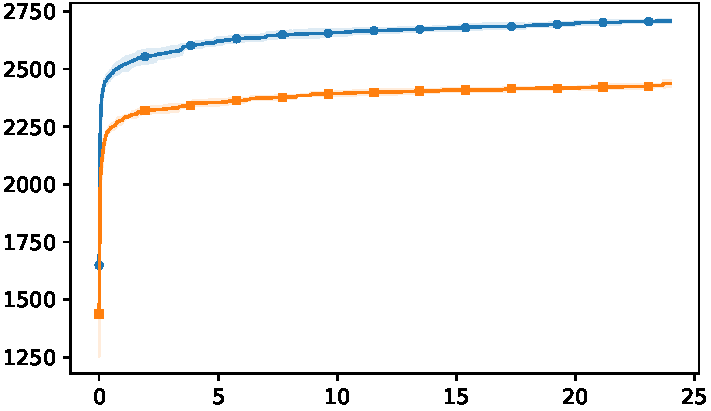
\includegraphics[width=\linewidth]{source/mosquitto.pdf}
\setlength{\abovecaptionskip}{-25pt} 
\setlength{\belowcaptionskip}{5pt}
\caption{mosquitto}
\end{subfigure}
\begin{subfigure}{0.49\textwidth}
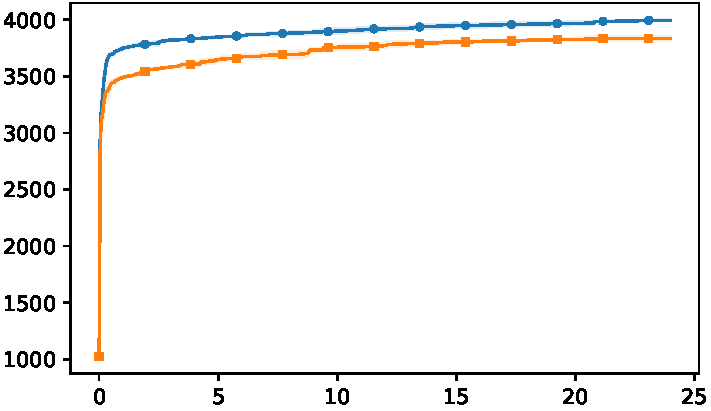
\includegraphics[width=\linewidth]{source/nanomq.pdf}
\setlength{\abovecaptionskip}{-25pt} 
\setlength{\belowcaptionskip}{5pt}
\caption{nanomq}
\end{subfigure}
\begin{subfigure}{0.49\textwidth}
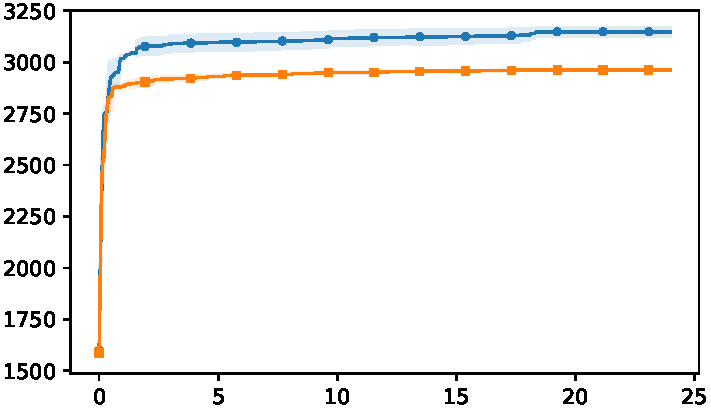
\includegraphics[width=\linewidth]{source/live555.pdf}
\setlength{\abovecaptionskip}{-25pt} 
\setlength{\belowcaptionskip}{5pt}
\caption{live555}
\end{subfigure}
\begin{subfigure}{0.49\textwidth}
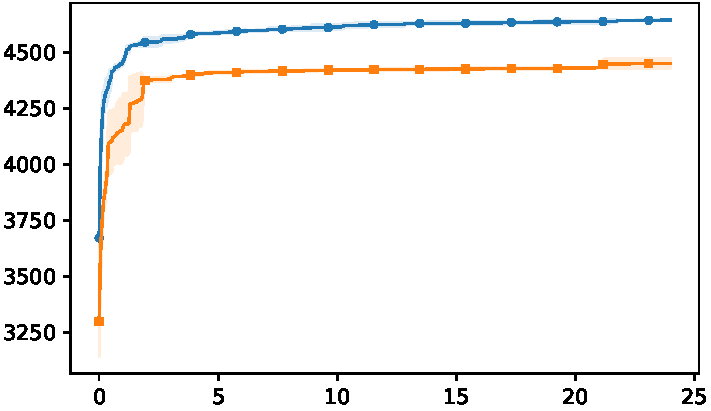
\includegraphics[width=\linewidth]{source/proftpd.pdf}
\setlength{\abovecaptionskip}{-25pt} 
\setlength{\belowcaptionskip}{5pt}
\caption{proftpd}
\end{subfigure}

\vspace{-5pt}
\begin{subfigure}{0.49\textwidth}
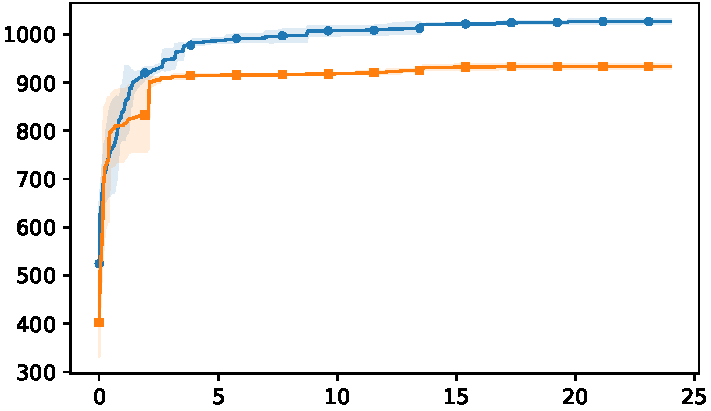
\includegraphics[width=\linewidth]{source/pure-ftpd.pdf}
\setlength{\abovecaptionskip}{-25pt} 
\setlength{\belowcaptionskip}{5pt}
\caption{pure-ftpd}
\end{subfigure}
\begin{subfigure}{0.49\textwidth}
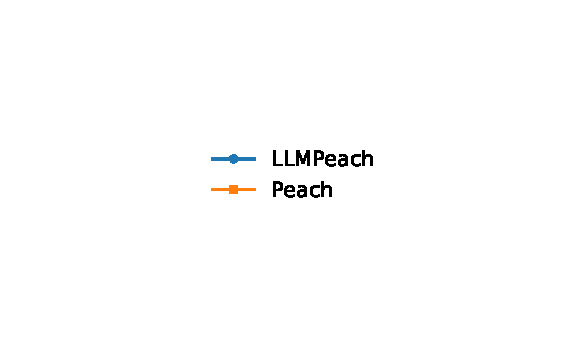
\includegraphics[width=\linewidth]{source/rq1_legend.pdf}
\setlength{\abovecaptionskip}{-25pt} 
\setlength{\belowcaptionskip}{5pt}
\caption*{}
\end{subfigure}

\vspace{-15pt}
{\zihao{5} \textbf{时间/小时}}
\end{minipage}

\bicaption{LLMPeach与Peach在分支覆盖上的变化趋势}{Trend of Branch Coverage between LLMPeach and Peach}
\label{fig:coverage_trend}
\end{figure}

观察发现，在测试的初始阶段（前 1-2 小时内），LLMPeach 和 Peach 在目标协议实现的分支覆盖上都呈现出快速增长的趋势，且 LLMPeach 在此阶段分支覆盖数上就已明显领先于 Peach。这表明 LLMPeach 生成的测试组件能够更快地触达协议实现中的关键分支，从而在测试初期就建立起更广泛的覆盖基础。随着测试时间的推移，LLMPeach 和 Peach 的分支覆盖增长速度逐渐趋于平缓，但 LLMPeach
的分支覆盖仍持续保持领先，并且在整个测试过程中都未出现被 Peach 反超的情况。此外，图中表示五次重复实验标准差的阴影区域整体较窄，说明LLMPeach在模糊测试中的表现具有较好的稳定性。

该结果表明，无论是进行短时间的快速测试，还是进行长时间的深度测试，LLMPeach 都能够持续地提供更高的分支覆盖，从而提升模糊测试的效果。


\section{RQ2:独特分支}

为了研究LLMPeach覆盖到的分支和Peach覆盖到的分支之间的关系，评估在多次实验中，LLMPeach覆盖到的分支中有多少是Peach始终未覆盖到的分支，本实验分析了两者在独特分支上的覆盖情况。

独特分支指的是在所有的实验轮次中，一种框架下被覆盖但在另一种框架下未被覆盖的分支。如果某个分支是 LLMPeach 覆盖到的独特分支，意味着该分支在所有5次Peach测试中都未被覆盖到；反之亦然。LLMPeach 覆盖到的独特分支数量越多，说明 LLMPeach 探索到了更多 Peach 始终未覆盖的分支；而Peach覆盖到的独特分支数量越多，则说明 LLMPeach 丢失了更多 Peach 原本能覆盖到的分支。

图 \ref{fig:venn} 展示了两者在独特分支上的对比结果，其中每个子图表示一个协议实现，左侧圆表示LLMPeach覆盖的分支，右侧圆表示Peach覆盖的分支，重叠部分表示两者都覆盖的分支，而非重叠部分则表示各自覆盖到的独特分支。

\begin{figure}[H]
\centering

\begin{subfigure}{0.32\textwidth}
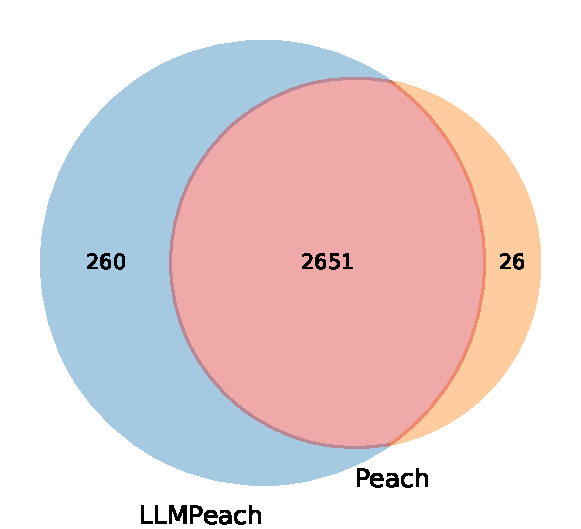
\includegraphics[width=\linewidth]{source/mosquitto-venn.pdf}
\setlength{\abovecaptionskip}{-20pt} 
\setlength{\belowcaptionskip}{5pt}
\caption{mosquitto}
\end{subfigure}
\begin{subfigure}{0.32\textwidth}
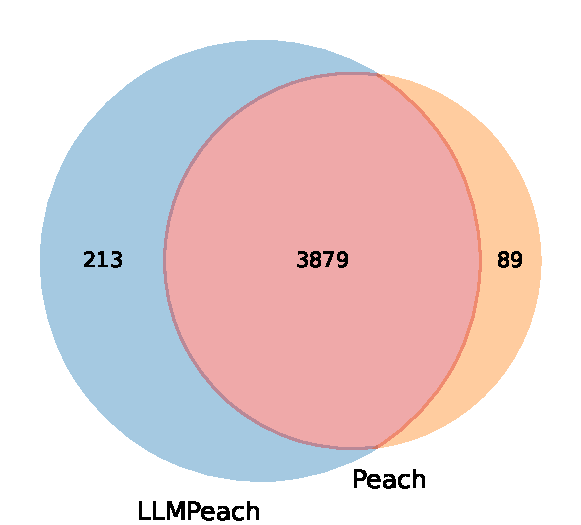
\includegraphics[width=\linewidth]{source/nanomq-venn.pdf}
\setlength{\abovecaptionskip}{-20pt} 
\setlength{\belowcaptionskip}{5pt}
\caption{nanomq}
\end{subfigure}
\begin{subfigure}{0.32\textwidth}
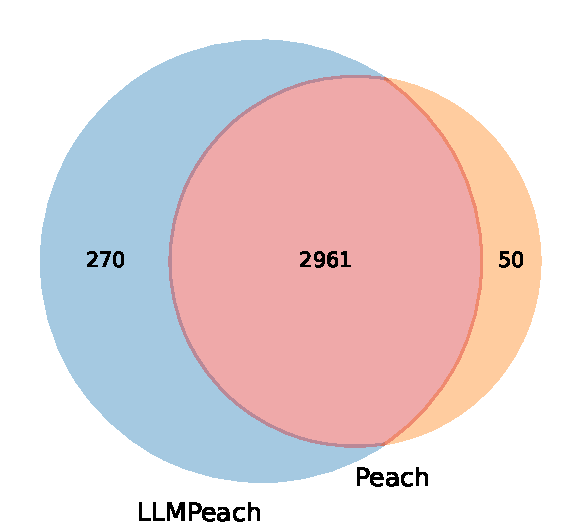
\includegraphics[width=\linewidth]{source/live555-venn.pdf}
\setlength{\abovecaptionskip}{-20pt} 
\setlength{\belowcaptionskip}{5pt}
\caption{live555}
\end{subfigure}
\begin{subfigure}{0.32\textwidth}
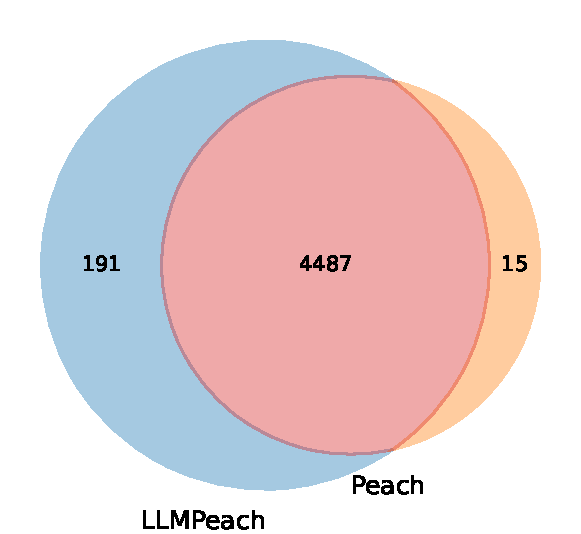
\includegraphics[width=\linewidth]{source/proftpd-venn.pdf}
\setlength{\abovecaptionskip}{-20pt} 
\setlength{\belowcaptionskip}{5pt}
\caption{proftpd}
\end{subfigure}
\vspace{-5pt}
\begin{subfigure}{0.32\textwidth}
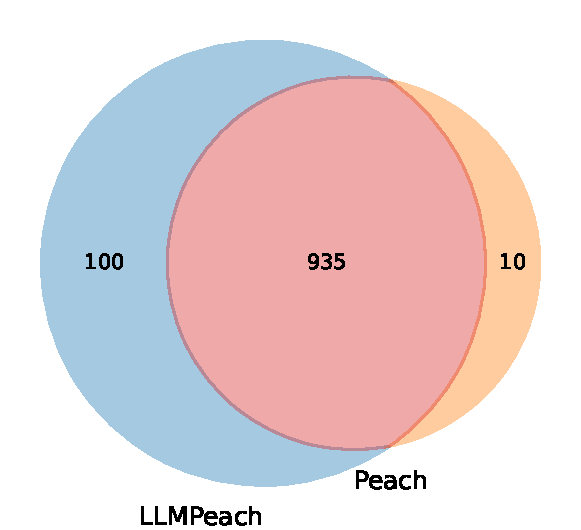
\includegraphics[width=\linewidth]{source/pure-ftpd-venn.pdf}
\setlength{\abovecaptionskip}{-20pt} 
\setlength{\belowcaptionskip}{5pt}
\caption{pure-ftpd}
\end{subfigure}
\begin{subfigure}{0.33\textwidth}
\end{subfigure}

\bicaption{LLMPeach与Peach在独特分支上的对比}{Comparison of Unique Branches between LLMPeach and Peach}
\label{fig:venn}
\end{figure}

实验数据显示，在所有被测协议中，LLMPeach 平均触发了206.8个独特分支，显著高于 Peach 框架的38个。在 mosquitto、proftpd和pure-ftpd中，Peach 的独特分支数量不足 LLMPeach 的10\%；而在 nanomq 和 live555 中，Peach 触发的独特分支数量虽然相对较多，但仍不及LLMPeach的50\%。这表明 LLMPeach 确实能够探索到大量 Peach 始终未覆盖的分支，且丢失的原本Peach能够覆盖到的分支数量非常有限，其收益远远大于损失。


\subsection{案例分析}

为了探究 LLMPeach 覆盖到的独特分支是否是与协议语义相关的分支，本文对其中一个协议实现 live555 中的独特分支进行了深入的案例分析。
该案例来自 \texttt{liveMedia/RTSPServer.cpp} 文件中的 \texttt{parseTransportHeader} 函数，
该函数负责解析 RTSP 请求中的 Transport 头部字段。图 \ref{fig:code} 展示了该函数中的一个代码片段，其中包含了多个条件分支来处理不同的 Transport 头部字段值。

\begin{figure}[H]
\centering
\begin{lstlisting}[numbers=left, frame=single, breaklines=true, basicstyle=\codefont\footnotesize, frameround=tttt,rulecolor=\color{black},backgroundcolor=\color{white},belowskip=0pt,numberstyle=\footnotesize\color{gray},
linebackgroundcolor={
    \ifnum\value{lstnumber}=4 \color{yellow}\fi
    \ifnum\value{lstnumber}=6 \color{yellow}\fi
}
]
static void parseTransportHeader(...) {
  // ...
  while (sscanf(fields, "%[^;\r\n]", field) == 1) {
    if (strcmp(field, "RTP/AVP/TCP") == 0) {
        streamingMode = RTP_TCP;
    } else if (_strncasecmp(field, "destination=", 12) == 0) {
        delete[] destinationAddressStr;
        destinationAddressStr = strDup(field+12);
    } // ...
  }
 // ...
}
\end{lstlisting}
\bicaption{live555中parseTransportHeader函数的代码片段}{Code Snippet of parseTransportHeader Function in live555}
\label{fig:code}
\end{figure}

在该函数中，LLMPeach 触发的其中独特分支位于第4行和第6行，分别对应于对 Transport 头部字段值的不同处理逻辑。
分析该函数的实现发现，这些独特分支与 RTSP 协议中 Transport 头部字段的语义相关。
例如，第4行的条件分支处理了当 Transport 头部字段值为 ``RTP/AVP/TCP" 时的情况，这是一种特定的传输模式；
而第6行的条件分支则处理了当 Transport 头部字段以 ``destination=" 开头时的情况，这涉及到目标地址的解析。

在 Pit 文件中，RTSP 请求的 Transport 头部字段的值被建模为一个字符串类型的参数。传统的 Peach 框架只能够知道该参数是一个字符串，但无法理解其内部的语义结构，因此在变异过程中可能会生成一些随机的字符串变异，难以触发上述条件分支；
而 LLMPeach 通过大语言模型的语义理解能力，能够识别出该参数的语义特征，并生成一些更具针对性的变异，例如变异为一些符合 RTSP 协议语义的字符串，其中
可能就包含了 ``RTP/AVP/TCP" 或者以 ``destination=" 开头的字符串，从而更有可能触发上述条件分支。

更进一步来说，当 live555 的 \texttt{parseTransportHeader} 函数解析 RTSP 请求中的 Transport 头部字段时，如果该字段的值为 ``RTP/AVP/TCP"，则会进入第5行的条件分支，设置 \texttt{streamingMode} 为 RTP\_TCP，这会导致后续的媒体流传输采用 RTP over TCP 的方式进行，从而触发更多与该传输模式相关的代码路径。这样，在后续的流程中，LLMPeach 便会触及到更多的独特分支。

通过以上案例分析，更进一步验证了 LLMPeach 覆盖到的独特分支确实是与协议语义相关的分支，这些分支的触发依赖于对协议参数的语义理解和针对性的变异生成，而这些正是 LLMPeach 相较于传统模糊测试工具的核心优势所在。

\section{RQ3: 两阶段变异策略}

为了评估 LLMPeach 中两阶段变异策略的效果，为探究两阶段变异策略对系统性能的贡献，通过对原策略进行替换与修改，构建了以下两种实验变体：
\begin{itemize}
    \item \textbf{LLMPeach$_{Random}$：}将两阶段变异策略替换为传统的随机策略，由随机策略调度LLM变异器和Peach内置变异器进行变异生成。
    \item \textbf{LLMPeach$_{LLMOnly}$：}仅使用大模型生成的变异器进行变异生成，完全去除Peach内置的变异器。
\end{itemize}

使用以上两个变体对五个协议实现进行模糊测试，
采取与之前相同的实验配置，每个工具运行24小时，并重复5次以获取平均结果。
表 \ref{tab:ablation}展示了两者在分支覆盖上和完整LLMPeach的对比。

\begin{table}[H]
\centering
\bicaption{LLMPeach与变体在分支覆盖上的对比}{Comparison of Branch Coverage between LLMPeach and Variants}
\label{tab:ablation}
\begin{tabular}{lccccc}
\toprule
\multirow{2}{*}{\textbf{协议实现}}
& \multirow{2}{*}{\textbf{LLMPeach分支覆盖}}   
& \multicolumn{2}{c}{\textbf{LLMPeach$_{Random}$}} 
& \multicolumn{2}{c}{\textbf{LLMPeach$_{LLMOnly}$}} \\
\cmidrule(lr){3-4} \cmidrule(lr){5-6}
& & \textbf{分支覆盖} & \textbf{变化} & \textbf{分支覆盖} & \textbf{变化} \\
\midrule
mosquitto & 2708.8 & 2638.0 & -2.61\% & 2611.6 & -3.59\% \\
nanomq    & 3994.4 & 3872.2 & -3.06\% & 3755.4 & -5.98\% \\
live555   & 3148.0 & 3076.4 & -2.27\% & 3026.2 & -3.87\% \\
proftpd   & 4643.2 & 4604.0 & -0.84\% & 4510.6 & -2.86\% \\
pure-ftpd & 1026.8 & 980.8  & -4.48\% & 901.0  & -12.25\% \\
\midrule
\textbf{平均} & -- & -- & \textbf{-2.65\%} & -- & \textbf{-5.71\%} \\
\bottomrule
\end{tabular}
\end{table}

\newpage

实验结果表明，LLMPeach$_{Random}$ 和 LLMPeach$_{LLMOnly}$ 在分支覆盖上均不如完整的 LLMPeach。LLMPeach$_{Random}$ 相较于 LLMPeach 平均分支覆盖下降了 2.65\%，而 LLMPeach$_{LLMOnly}$ 的平均分支覆盖下降幅度更大，达到了 5.71\%。

LLMPeach$_{LLMOnly}$ 效果的下降说明，如果仅采用大模型生成的语义相关的变异器，而不结合传统的变异器进行随机的变异探索，整体的分支覆盖效果会显著下降。这表明两阶段变异策略中的第二阶段，在提升分支覆盖方面同样发挥了作用。可能是因为第一阶段生成的语义相关变异器虽然能够触发一些特定的分支，但如果没有第二阶段的Peach变异器来提供更多样化的变异输入，测试用例的多样性和覆盖范围就会受到限制，从而导致整体分支覆盖率的下降。这说明两阶段变异策略中保留Peach内置变异器是有意义的。

而 LLMPeach$_{Random}$ 的效果下降则说明，如果仅仅加入大模型生成的测试组件，简单地将LLM变异器和Peach变异器放在一起进行随机调度，而不采用两阶段变异策略来引导变异生成的流程，整体的分支覆盖效果同样会下降。这表明将变异生成过程划分为两个阶段，在第一阶段进行语义相关的变异，第二阶段辅以随机的变异探索，而不是仅仅将两者混合在一起进行简单的扩充，这样的设计是有益于测试效果的。

图 \ref{fig:coverage_trend_3} 展示了 LLMPeach 与两个变体在分支覆盖上的变化趋势。

在测试的绝大多数时间段内，LLMPeach 的分支覆盖数量始终领先于两个变体，并在领先以后的时间段内持续保持领先。这表明两阶段变异策略能够在测试的不同阶段持续地提供更高效的变异输入，从而提升分支覆盖率。

此外，还可以发现，如子图(c)(d)(f)所示，在一些协议实现上，在测试的前1-2小时，LLMPeach$_{LLMOnly}$ 的分支覆盖数量与 LLMPeach 的分支覆盖数量相近，甚至在某些时间点上略微领先于 LLMPeach。这表明在测试的初始阶段，第一阶段的语义相关变异生成策略能够提供一些有针对性的变异输入，从而触发一些特定的分支；但随着测试的进行，第二阶段的随机变异生成策略开始发挥作用，提供更多样化的变异输入，从而使得 LLMPeach 的分支覆盖率逐渐拉开与 LLMPeach$_{LLMOnly}$ 的差距。

此部份实验表明，为大模型生成的语义相关的测试组件设计两阶段变异策略，既能够利用语义相关变异器来触发一些特定的分支，又能够通过随机的变异生成策略来提供更多样化的变异输入，从而在整体上提升分支覆盖率，是一种有效的设计选择。


\begin{figure}[H]
\centering

\begin{minipage}[c]{0.04\textwidth}
\centering
\rotatebox[origin=c]{90}{{\zihao{5} \textbf{分支覆盖}}}
\end{minipage}
\hfill
\begin{minipage}[c]{0.95\textwidth}
\centering

\begin{subfigure}{0.49\textwidth}
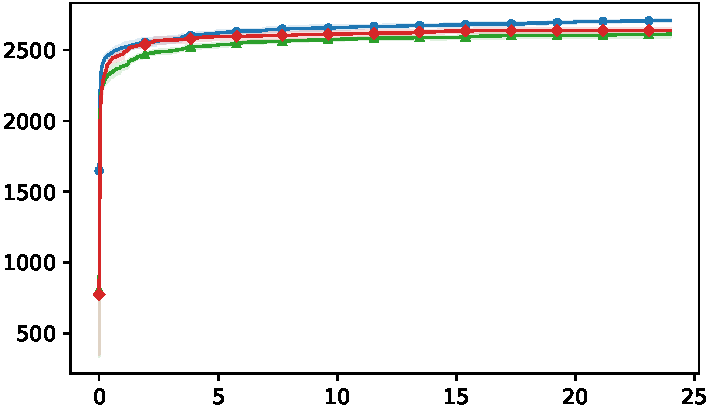
\includegraphics[width=\linewidth]{source/mosquitto-3.pdf}
\setlength{\abovecaptionskip}{-25pt} 
\setlength{\belowcaptionskip}{5pt}
\caption{mosquitto}
\end{subfigure}
\begin{subfigure}{0.49\textwidth}
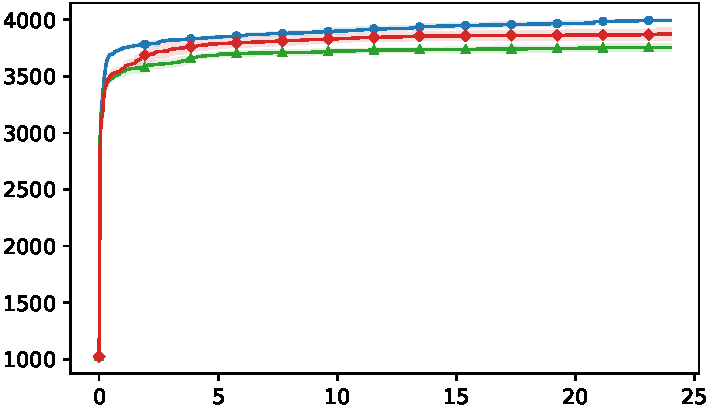
\includegraphics[width=\linewidth]{source/nanomq-3.pdf}
\setlength{\abovecaptionskip}{-25pt} 
\setlength{\belowcaptionskip}{5pt}
\caption{nanomq}
\end{subfigure}
\begin{subfigure}{0.49\textwidth}
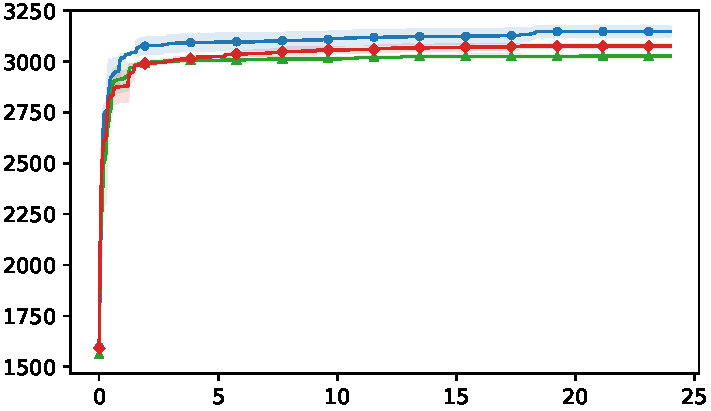
\includegraphics[width=\linewidth]{source/live555-3.pdf}
\setlength{\abovecaptionskip}{-25pt} 
\setlength{\belowcaptionskip}{5pt}
\caption{live555}
\end{subfigure}
\begin{subfigure}{0.49\textwidth}
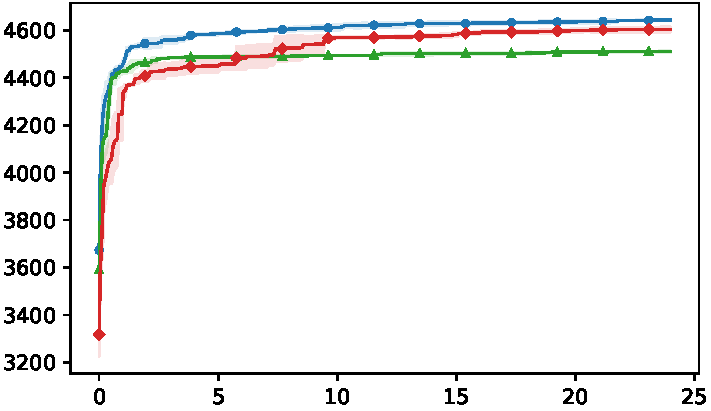
\includegraphics[width=\linewidth]{source/proftpd-3.pdf}
\setlength{\abovecaptionskip}{-25pt} 
\setlength{\belowcaptionskip}{5pt}
\caption{proftpd}
\end{subfigure}

\vspace{-5pt}
\begin{subfigure}{0.49\textwidth}
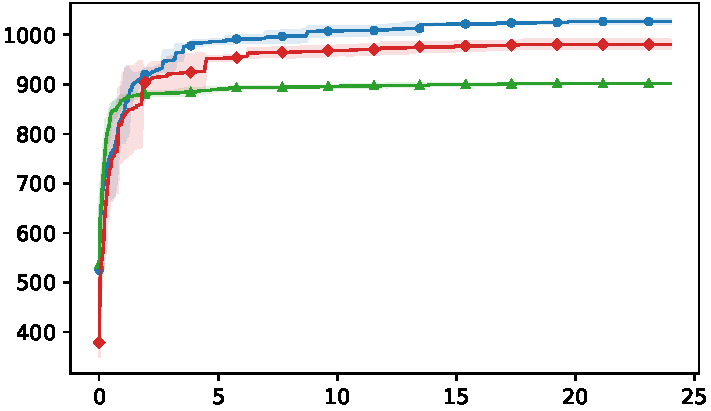
\includegraphics[width=\linewidth]{source/pure-ftpd-3.pdf}
\setlength{\abovecaptionskip}{-25pt} 
\setlength{\belowcaptionskip}{5pt}
\caption{pure-ftpd}
\end{subfigure}
\begin{subfigure}{0.49\textwidth}
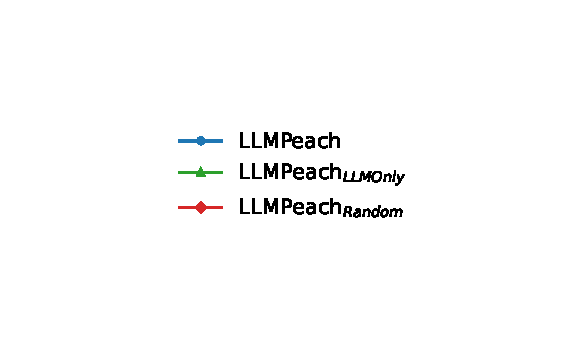
\includegraphics[width=\linewidth]{source/rq3_legend.pdf}
\setlength{\abovecaptionskip}{-25pt} 
\setlength{\belowcaptionskip}{5pt}
\caption*{}
\end{subfigure}

\vspace{-15pt}
{\zihao{5} \textbf{时间/小时}}
\end{minipage}

\bicaption{LLMPeach与变体在分支覆盖上的变化趋势}{Trend of Branch Coverage between LLMPeach and Variants}
\label{fig:coverage_trend_3}
\end{figure}

% \begin{figure}[H]
% \centering

% \begin{subfigure}{0.32\textwidth}
% 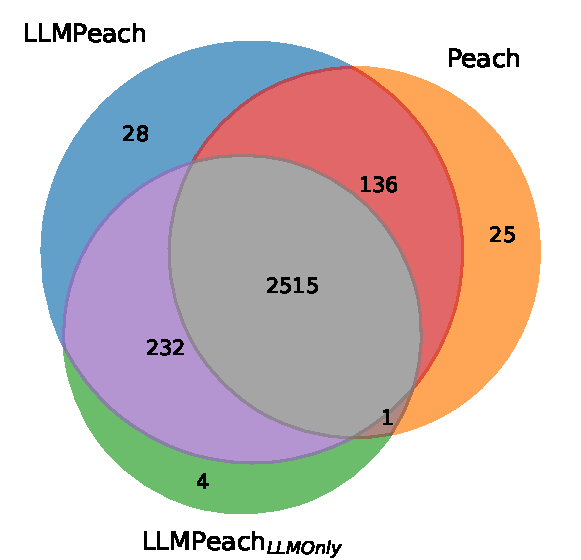
\includegraphics[width=\linewidth]{source/mosquitto-venn-3.pdf}
% \setlength{\abovecaptionskip}{-20pt} 
% \setlength{\belowcaptionskip}{5pt}
% \caption{mosquitto}
% \end{subfigure}
% \begin{subfigure}{0.32\textwidth}
% 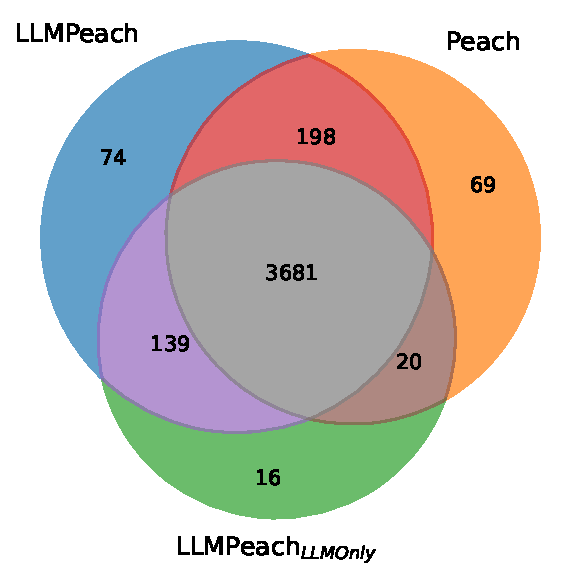
\includegraphics[width=\linewidth]{source/nanomq-venn-3.pdf}
% \setlength{\abovecaptionskip}{-20pt} 
% \setlength{\belowcaptionskip}{5pt}
% \caption{nanomq}
% \end{subfigure}
% \begin{subfigure}{0.32\textwidth}
% 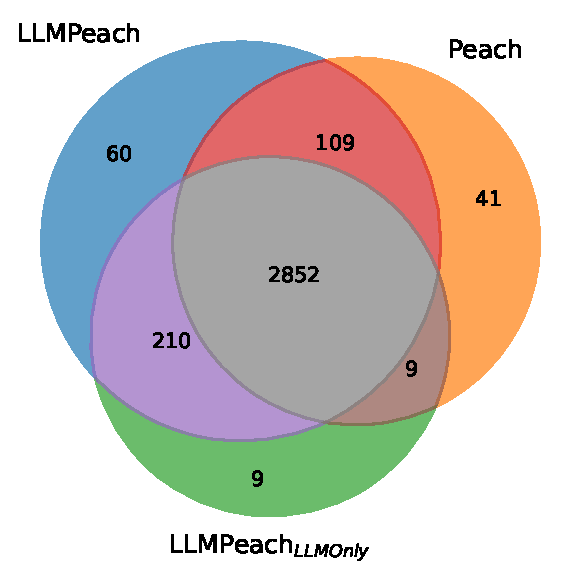
\includegraphics[width=\linewidth]{source/live555-venn-3.pdf}
% \setlength{\abovecaptionskip}{-20pt} 
% \setlength{\belowcaptionskip}{5pt}
% \caption{live555}
% \end{subfigure}
% \begin{subfigure}{0.32\textwidth}
% 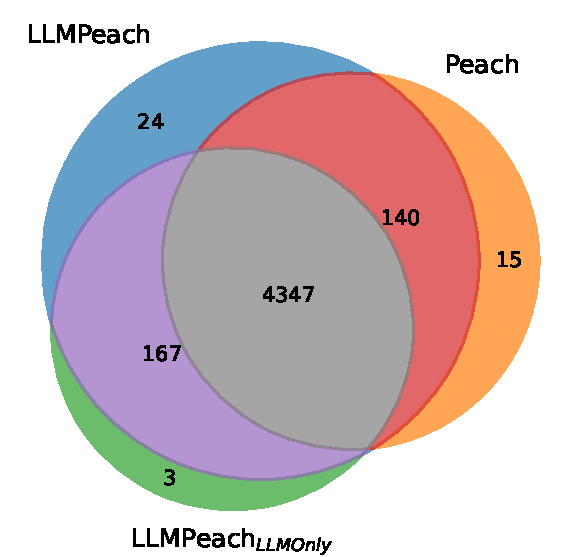
\includegraphics[width=\linewidth]{source/proftpd-venn-3.pdf}
% \setlength{\abovecaptionskip}{-20pt} 
% \setlength{\belowcaptionskip}{5pt}
% \caption{proftpd}
% \end{subfigure}
% \vspace{-5pt}
% \begin{subfigure}{0.32\textwidth}
% 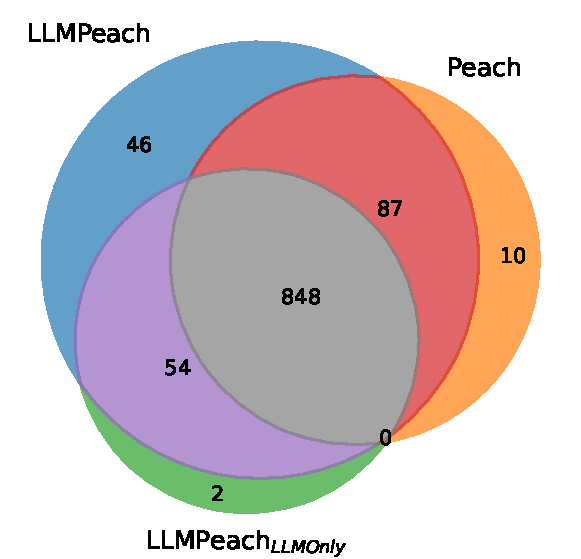
\includegraphics[width=\linewidth]{source/pure-ftpd-venn-3.pdf}
% \setlength{\abovecaptionskip}{-20pt} 
% \setlength{\belowcaptionskip}{5pt}
% \caption{pure-ftpd}
% \end{subfigure}
% \begin{subfigure}{0.33\textwidth}
% \end{subfigure}

% \end{figure}
